\documentclass[11pt]{report}

\usepackage{geometry}
 \geometry{
 a4paper,
 total={210mm,297mm},
 left=25mm,
 right=25mm,
 top=30mm,
 bottom=25mm,
 headsep=7mm}

\interfootnotelinepenalty=10000

\usepackage[dvipsnames]{xcolor}
\usepackage{graphicx}
\usepackage{titlesec}
\usepackage{todonotes}
\usepackage{float}
\usepackage[hidelinks]{hyperref}
\usepackage{listings}
\usepackage{enumerate}
\usepackage{fancyhdr}
\usepackage{longtable}
\usepackage{microtype}
\usepackage{dirtree}

\graphicspath{ {images/} }

\pagestyle{fancy}
\fancyhf{}
\fancyhead[L]{\leftmark}
\fancyfoot[C]{\thepage}
\renewcommand{\headrulewidth}{0.4pt}

\begin{document}

	\begin{titlepage}
		\centering
		
\includegraphics{logo.png}\par\vspace{1cm}
		{\scshape\LARGE\bfseries Politecnico di Milano \par}
		\vspace{1cm}
		{\scshape\Large Software Engineering 2\par}
		\vspace{1.5cm}
		{\Huge\bfseries Implementation and Test document\par}
		\vspace{1cm}
		{\small Version 1.0 - 30/12/2017\par}
		\vspace{1cm}
		{\normalsize\href{https://github.com/JustSalva/MelziPinaSalvadore/tree/master/DeliveryFolder}{\color{blue}Installation link}\par} 
		\vspace{0.5cm}
		{\href{https://github.com/JustSalva/MelziPinaSalvadore/tree/master/Implementation/ApplicationServer}{\color{blue}Application server source code link}\par} 
		\vspace{0.5cm}
		{\href{https://github.com/JustSalva/MelziPinaSalvadore/tree/master/Implementation/AndroidApp/Travlendar}{\color{blue}Android app source code link}\par} 
		\todo{TODO}
		\vspace{4cm}
		{\Large\itshape Pietro Melzi, Alessandro Pina, Matteo Salvadore\par}

		\vfill

		% Bottom of the page
		{\large AA 2017-2018\par}
	\end{titlepage}

	\tableofcontents{}

	\chapter{INTRODUCTION}
	\label{ch:INTRODUCTION}
	
		\section{Purpose}
		\label{sect:Purpose}
			\todo{TODO}
			
		\section{Scope}
		\label{sect:Scope}
			Travlendar+ is a service based on a mobile application.\\
The system aims to help his users with a calendar-based application that support the users, computing travels between his events, helping them to organize their schedule and allowing them to arrange their trips. \\ 
For further details see the Scope section in the RASD document.
			
		\section{Definitions, Acronyms, Abbreviations}
		\label{sect:Definitions, Acronyms, Abbreviations}
			\subsection{Definitions}
	\begin{itemize}
	\item \textit{Arrange trip}: the system provides all the information available about a travel to the user. If the travel is related to one or more public travel means, the system helps the user to organize it. It is indicated if the user already holds a valid ticket for a certain travel or if he has to buy a required one. Purchase of a ticket is handled on the websites of the transport service providers. Trip and travel are synonymous.
	\item \textit{Best path}: it is the preferred travel option proposed to reach the event location among all the feasible paths, according to parameters specified by the user. The best path can be chosen according to one of these features: length, cost or environmental sustainability. Best path is the path taken into account and showed in the daily schedule; the user can substitute it at any moment with an alternative feasible path. 
	\item \textit{Break event}: it is an optional event whose starting and ending time are flexible. The user can define this kind of event when he wants to reserve a certain amount of time in the schedule and he doesn't need to specify a starting time. For instance, a user could be able to specify that lunch must be possible every day between 11:30-
2:30, and it must be at least half an hour long, but the specific timing is flexible. The app would then be sure to reserve, if possible, at least 30 minutes for lunch each day.
	\item \textit{Constraint}: it is a rule defined on travel means by the user. When the system calculates feasible paths, each constraint must be taken into account: travel options not respectful of existing constraints are ignored. A constraint can be associated to a type of event. 
	\newline
	There are different types of constraints: min/max distance allowed for a travel mean, interval of hours in which it is possible to take a travel mean and possibility to deactivate a travel mean. 
	\item \textit{Customized type of event}: it is a set of rules related to a particular type of event that can be used several time by the user. The user can define a customized type of event in hs preferences, starting from the default type of event.	
	\item \textit{Default type of event}: it is a general set of rules defined usually the first time that the user exploits the system, it can be modified. Default type of event is related to each event that doesn't need a particular type of event. New types of event are defined starting from the constraints enclosed in the default one.	
	\item \textit{Feasible path}: a path that allows the user to reach a specified location before the starting time of the event to attend. It observes the constraints defined for that event.
	\item \textit{Google Maps API}: a set of functions offered by Google Maps to decide the travel path between two locations.
	\item \textit{Overlapping event}: an event (or a part of it) that happens in the same time slot of another event, added previously in the schedule. Because the schedule must be feasible, an event is considered as "overlapping" also if only its related travel overlaps an event present in the schedule.
	\item \textit{Periodicity}: it is related to events that occur more than one time. It can be defined as weekly, monthly or in which days of the week the event happen.
	\item \textit{Schedule}: a daily plan containing a set of events inserted by the user that allows him to travel and attend all the events. If an event overlaps other events, it cannot be inserted into the schedule. 
	\item \textit{Type of event}: a set of rules (constraints) that is defined by the user and can be associated to multiple events.
	\item \textit{Transport service provider}: a public or private company that controls and supplies the transport with a travel mean. 
	\item \textit{Travel}: it is used to indicate the path that the user has to follows in order to reach a location. It can be composed by different travel components.
	\item \textit{Travel component}: each single path that can be traveled with a travel mean. It has a starting time, a ending time, a departure location, an arrival location and a length. The union of one or more travel components creates a travel.
	\end{itemize}
			\subsection{Acronyms}
	\begin{itemize}
	\item \textit{API}: Application Programming Interface;
	\item \textit{ACID}: Atomicity, Consistency, Isolation and Durability;
	\item \textit{DB}: Data Base;
	\item \textit{DBMS}: Data Base Management System;
	\item \textit{DD}: Design Document;
	\item \textit{GCM}: Google Cloud Messaging;
	\item \textit{GTFS}: General Transit Feed Specification;
	\item \textit{HTTP}: HyperText Transfer Protocol;
	\item \textit{ICSEA}: Tenth International Conference on Software Engineering Advances;
	\item \textit{ITD}: Implementation and Test Document;
	\item \textit{Java EE}: Java Enterprise Edition;
	\item \textit{RASD}: Requirement Analysis and Specification Document;
	\item \textit{RESTful}: REpresentational State Transfer;
	\item \textit{RSA}: Rivest-Shamir-Adleman algorithm;
	\item \textit{UTC}: Coordinated Universal Time.
	\end{itemize}
			\subsection{Abbreviations}
	\begin{itemize}
   	\item \textit{TSP}: Transport Service Provider. 
	\end{itemize}
\todo{TODO}
			
		\section{Revision history}
		\label{sect:Revision history}
			2017/11/26 - \textit{Version 1.0} - First delivery of DD.
			
		\section{Reference Documents}
		\label{sect:Documents}
			\begin{itemize}
\item Specification Document: "Mandatory Project Assignments.pdf";
\item Specification Document: "Implementation and Testing Assignments.pdf";
\item Requirements Analysis and Specification Document, version 1.1;
\item Design Document, version 1.1.
\end{itemize}
			
		\section{Document Structure}
		\label{sect:Document Structure}
			This Design Document is composed by eight chapters:
\begin{enumerate}
\item The first chapter is an introduction to DD and contains also other information: definition of the used terms, revision history of the document and references;
\item The second chapter is dedicated to the architecture of the system. In this section is given a description of different components, providing information on their deployment, on the offered functionalities and on the interaction between them. The last section of the chapter explains techniques and design decisions used to realize several aspects of the system;
\item The third chapter includes a general description of the main algorithms to be used by the system-to-be;
\item The fourth chapter explains how the user can interact with the system: here are shown mockups and user experience diagrams;
\item The fifth chapter contains a table that explains the relations between a component of the system and the requirements that this component satisfies.
\item The sixth chapter refers to the realization phase of the product: it describes and establishes rules of precedence for implementation, integration and testing of the system;
\item The seventh chapter contains a report of the hours spent to write this document;
\item The eighth chapter contains references to external documents used in this document and to the software used in order to write this document.
\end{enumerate}

			
	\chapter{IMPLEMENTED REQUIREMENTS}
	\label{ch:IMPLEMENTED REQUIREMENTS}
		Our first release of Travlendar+ includes all core functionalities of the application server and of the database server, as specified in the previous documents (more details in section \ref{sec:ApplAndDBServers}), a set of initial functionalities in the Android application (more details in section \ref{sec:AndroidApp}) and does not include neither the web server implementation or the IOs app.
In the following schema we have highlighted the components of our general architecture (see also section 2.1 of DD) that are actually implemented and tested (components are encircled in green, the integration of the subsystems are colored in green). As stated before, in the following sections we will explain in details what exactly has been implemented.
\begin{figure}[H]
	\begin{center}
		\hspace*{-40pt}
		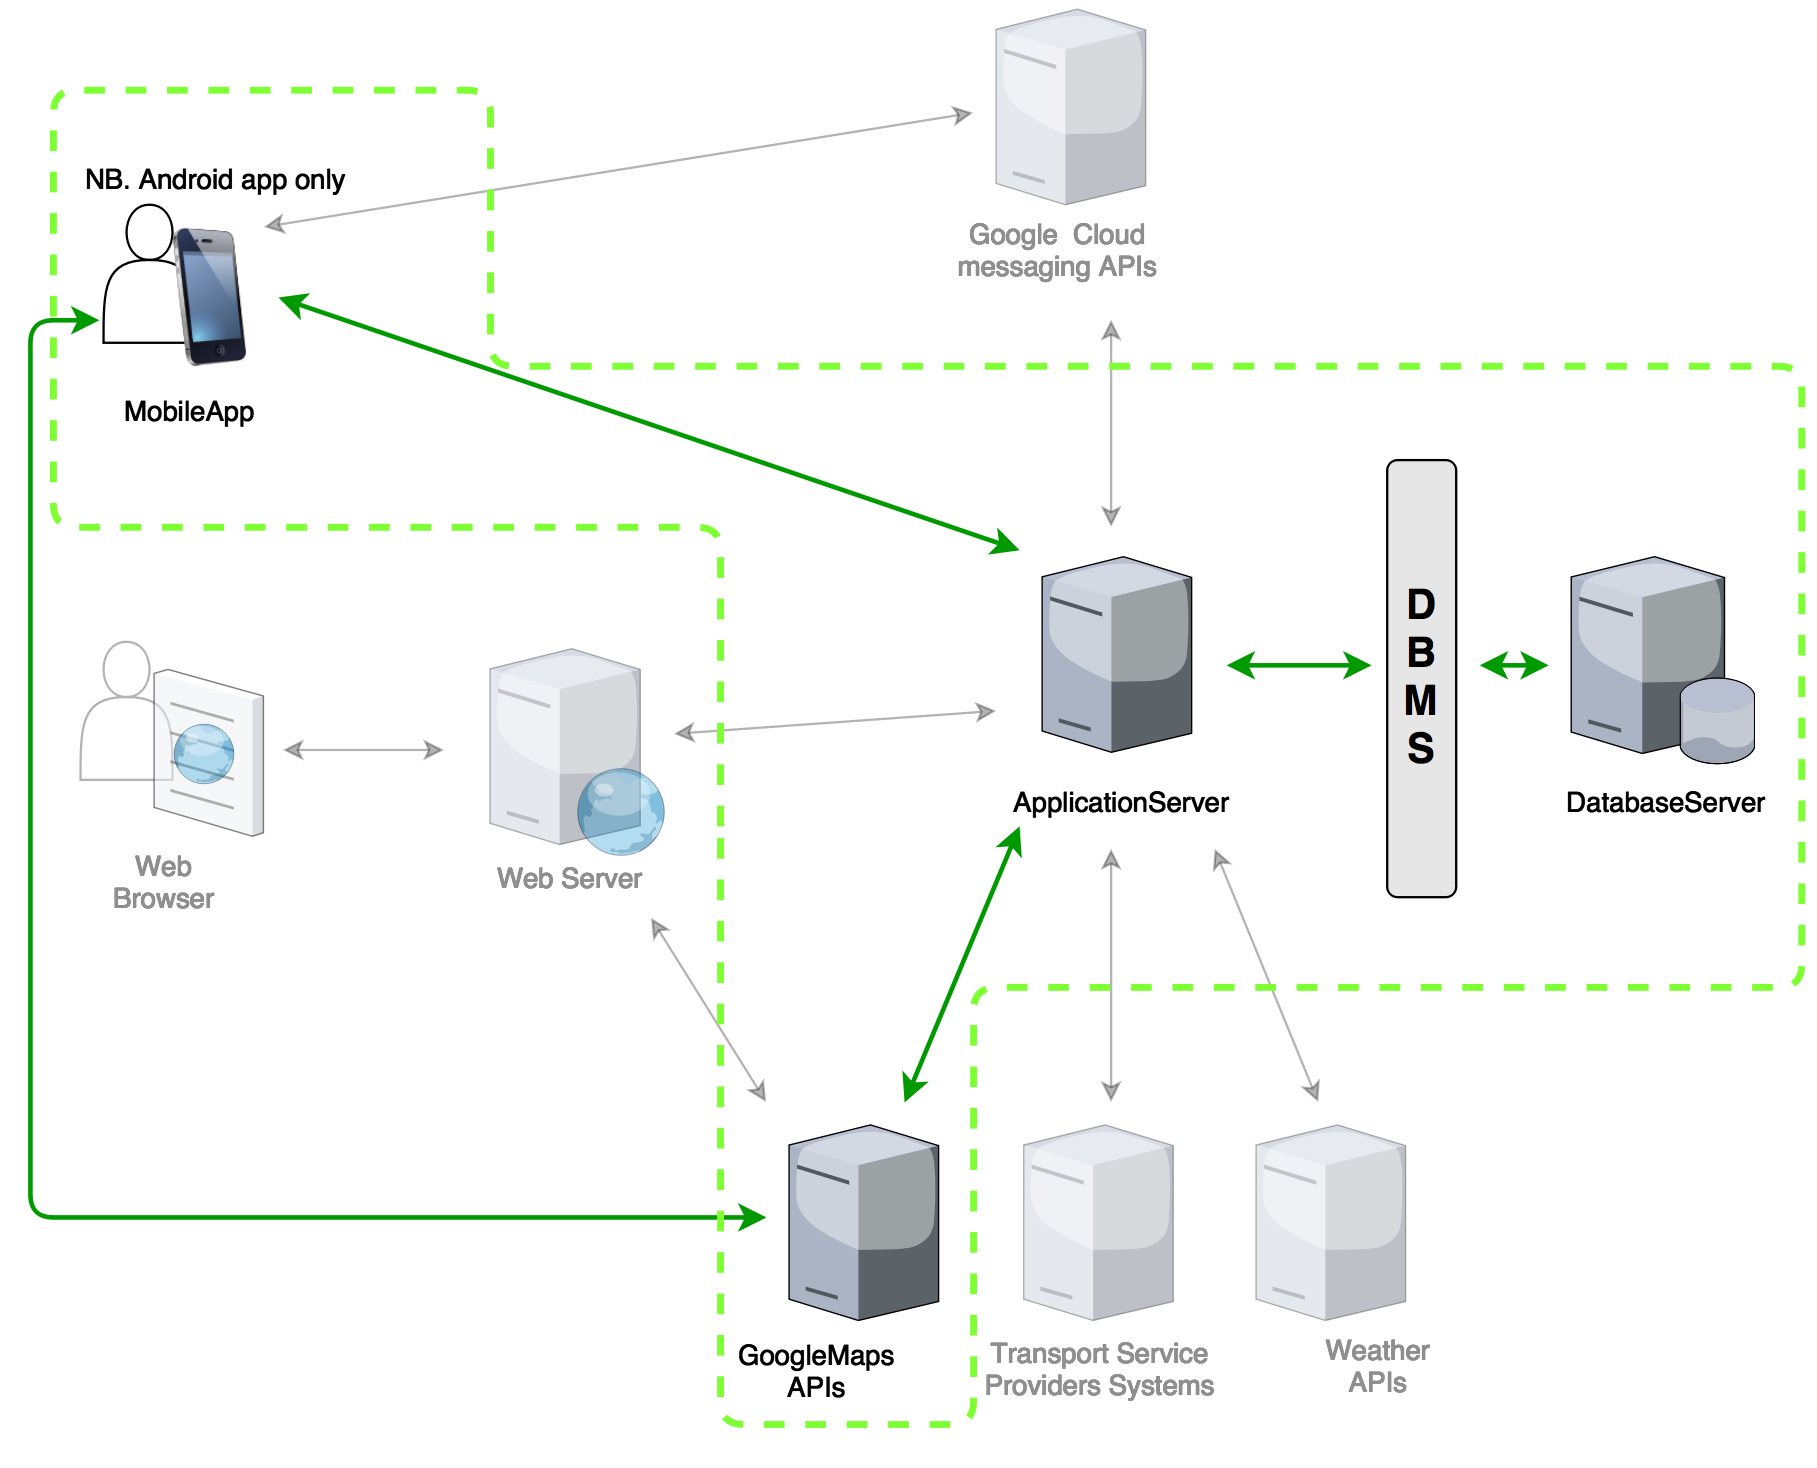
\includegraphics[scale=0.2]{GeneralArchitecture.png}
	\end{center}
\caption{General Architecture - Implemented subsystems}
\end{figure}

\newpage

\noindent Our software includes all the functionalities that:
\begin{itemize}
	\item Allow the users to have a calendar of events which can be either scheduled or non scheduled;
	\item Compute feasible travels which allow the users to reach their scheduled events in the allotted time;
	\item Allow the users to define their own preference profiles, which are to be applied to the travels proposed by our system;
	\item Allow the users to save their preferred locations into their profiles;
	\item Allow the users to define flexible breaks and to define periodical events;
	\item Allow the users to save their tickets and associate them to compatible travel components.
\end{itemize}
\noindent 
In this first release are not included the functionalities that:
\begin{itemize}
	\item Allow the users to buy new tickets within our application;
	\item Allow the users to locate the nearest sharing vehicles;
	\item Allow the system to take into account weather, forecast, strikes and traffic info and to notify the user if a path is no more feasible due to those issues.
\end{itemize} 
We have decided not to include them in our first release since we consider them as nice-to-have feature, but not mandatory for an initial release. They depend on other functionalities we have implemented and so they must come after those functionalities. We had then to choose how to allocate properly the limited amount of time given for the implementation phase and those functionalities would have required more time to be implemented. \\
Here we provide a list of use cases, taken from our RASD document (section 3.2.3) that are satisfied in this first release:
\begin{itemize}
	\item [UC1] Registration;
	\item [UC2] Login;
	\item [UC3] View calendar;
	\item [UC4] Create event;
	\item [UC5] Create personalized event profiles;
	\item [UC6] Define flexible breaks;
	\item [UC7] Arrange trips - Only with ticket inserted by the user;
	\item [UC9] Add ticket possessed;
	\item [UC10] Obtain feasible travel paths - Without the alternatives paths;
	\item [UC11] Choose between overlapping events;
	\item [UC12] Edit event - Only in Application server, not yet available on Android app; 
	\item [UC13] Delete event;
	\item [UC14] Edit personalized event profiles;
	\item [UC15] Delete personalized event profiles.
\end{itemize}

\section{Application Server and Database Server}
\label{sec:ApplAndDBServers}
In this section we specify which requirements are actually implemented in our ApplicationServer subsystem, examining every sub-component, and stating which requirements are implemented in this first release of Travlendar+. We also state the motivations for including them and excluding others (see also chapter 5 of DD - requirement traceability).
\begin{figure}[H]
	\begin{center}
		\hspace*{-60pt}
		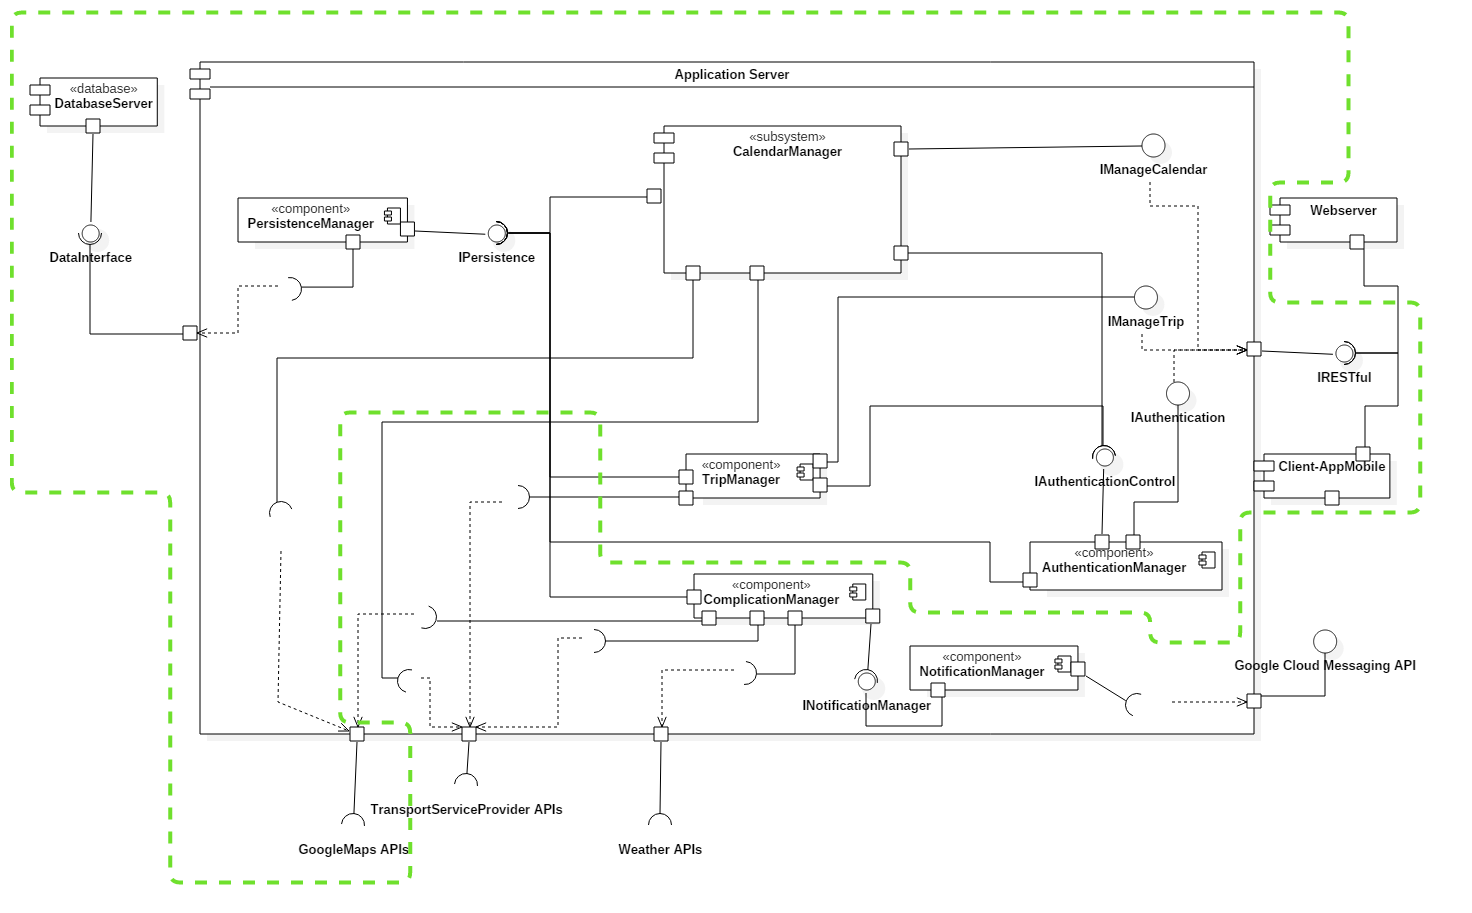
\includegraphics[scale=0.4]{ApplicationServer.png}
	\end{center}
\caption{The implemented components of the Application Server}
\end{figure}

\subsection{Authentication Manager}
All the requirements related to the authentication manager are fulfilled in this first release: the user can register himself into the system, log in from any device he prefers (but only one at the time), modify his account's info, delete his account and request a new password. \\
As specified in the previous documents, these are the requirements met by this manager:
\begin{itemize}
	\item \textbf{[R1]} the system checks if the e-mail inserted is real;
	\item \textbf{[R2]} a user cannot sign up with the same e-mail twice;
	\item \textbf{[R3]} the e-mail and password inserted must be correct;
	\item \textbf{[R4]} incorrect credentials prevent the user from logging in;
	\item \textbf{[R38]} a user must be logged.
\end{itemize}

\subsection{Event Manager}
Event manager handles insertion, deletion and modification of both events and break events into the user's calendar.
It interacts with both path and schedule manager in order to provide feasible paths to the events and to decide whether they can be scheduled or not.
In the application server also the propagation of periodical events through the time is handled properly. \\
In our system is not yet handled the possibility to modify and delete with one operation all the periodic events generated from one single event, due to time-related issues.
In our system is not yet handled the possibility to define events without an ending time since we do not consider this feature essential, but just an optional and not so necessary feature. \\
As specified in the previous documents, these are the requirements met by this manager:
\begin{itemize}
	\item \textbf{[R5]} a user must specify all mandatory fields to add the new event;
	\item \textbf{[R6]} the system reserves the specified time-slot for the event;
	\item \textbf{[R7]} the system warns the user if the inserted event overlaps with an already existing one;
	\item \textbf{[R29]} the system allows the user to specify a flexible interval and a minimum amount of time to schedule a break.
\end{itemize}
And these are the requirements not yet implemented in this manager:
\begin{itemize}
	\item \textbf{[R8]} if the ending time of an event is not specified, the systems considers as ending time the hour of departure for the successive event;
	\item \textbf{[R9]} when an event is inserted after an event without a specified ending time, the ending time  of the first event is anticipated as stated in [R8].
\end{itemize}

\subsection{Preference Manager}
All the requirements related to the preference manager are fulfilled.
This module offers all the functionalities needed to insert, modify and delete the user's event profiles and the user's preferred locations. It is also able to apply the user's preferences to the feasible travels computed by our system. \\
As specified in the previous documents, these are the requirements met by this manager:
\begin{itemize}
	\item \textbf{[R12]} the system does not consider paths that violate constraints on travel means defined by the user;
	\item \textbf{[R13]} the system checks user preferences to decide which feasible travel path is the best;
	\item \textbf{[R15]} appropriate travel means must be suggested according to the type of event that they are related to;
	\item  \textbf{[R23]} the system requires minimum and maximum length allowed for a path to impose a constraint on a travel mean;
	\item \textbf{[R24]} the system requires an interval of time allowed to impose a constraint on a travel mean;
	\item \textbf{[R25]} the system does not consider solutions that violate constraints;
	\item \textbf{[R26]} the system allows the user to specify one or more travel means that cannot be used;
	\item \textbf{[R27]} the system does not consider solutions that include deactivated travel means.
\end{itemize}

\subsection{Path Manager}
This module manages the feasible travels computation, after the insertion or the modification of an event. It interacts with the \textit{PreferenceManager} in order to obtain the information needed to guarantee that the user preferences are respected in every proposed path.\\
The functionalities that allow to change a selected path, choosing between a set of feasible alternatives, to obtain info that allow to draw a feasible path on a map and to obtain also options that include sharing vehicles are not yet available; we've chosen not to include them due to time-related issues and because they would have been nice-to-have features but not essential for an initial release. \\
As specified in the previous documents, these are the requirements met by this manager:
\begin{itemize}
	\item \textbf{[R10]} every travel path proposed must be feasible in the available time (the interval between two consecutive events);
	\item \textbf{[R11]} if the travel involves two or more travel means, the starting location of the first proposed travel path and the ending location of the last proposed travel path must coincide respectively with the starting location and the ending location of the whole planned travel;
	\item \textbf{[R12]} the system does not consider paths that violate constraints on travel means defined by the user;
	\item \textbf{[R13]} the system checks user preferences to decide which feasible travel path is the best;
	\item \textbf{[R15]} appropriate travel means must be suggested according to the type of event that they are related to;
	\item \textbf{[R25]} the system does not consider solutions that violate constraints;
	\item \textbf{[R27]} the system does not consider solutions that include deactivated travel means;
	\item \textbf{[R35]} the system provides information about time of departure and arrival of the proposed travels.
\end{itemize}
And these are the requirements not yet implemented in this manager:
\begin{itemize}
	\item \textbf{[R18]} the system must show to the user all possibilities to reach a location in according with the requirements of [G4];
	\item \textbf{[R19]} alternative feasible travel paths must not generate overlappings with other events of the schedule;
	\item \textbf{[R28]} for each travel path, the system estimates its carbon footprint produced;
	\item \textbf{[R37]} the system provides information about travel time with shared vehicles.
\end{itemize}

\subsection{Schedule Manager}
This module is able to check if an event overlaps with other events and to guarantee that the flexible breaks are respected. It also checks that the user's travels do not overlap with other events. When an event overlaps with another one, the schedule manager puts it in a separate list of non scheduled events and it manages the user's requests of rescheduling those events. \\
As specified in the previous sections, events without an ending time and alternative travels are not yet implemented into our system since, due to time-related issues, we've decided to exclude them from our first release of Travlendar+. \\
As specified in the previous documents, these are the requirements met by this manager:
\begin{itemize}
	\item \textbf{[R6]} the system reserves the specified time-slot for the event;
	\item \textbf{[R7]} the system warns the user if the inserted event overlaps with an already existing one;
	\item \textbf{[R14]} the system warns the user if it is not possible to arrive at an event location before its starting time;
	\item \textbf{[R20]} the combination of the travel paths proposed for the day must be feasible in the allotted time;
	\item \textbf{[R21]} if there are multiple events at the same time the system will propose in the schedule only the first event added;
	\item \textbf{[R22]} if the user forces into the schedule an event that overlaps with events already present in the schedule, these are removed from the schedule;
	\item \textbf{[R30]} if there is enough time for a break, the system reserves it within the specified flexible interval;
	\item \textbf{[R31]} if there is not enough time into the flexible interval specified, a warning is thrown.
\end{itemize}

And these are the requirements not yet implemented in this manager:
\begin{itemize}
	\item \textbf{[R8]} if the ending time of an event is not specified, the systems considers as ending time the hour of departure for the successive event;
	\item \textbf{[R9]} when an event is inserted after an event without a specified ending time, the ending time  of the first event is anticipated as stated in [R8];
	\item \textbf{[R19]} alternative feasible travel paths must not generate overlappings with other events of the schedule.
\end{itemize}

\subsection{Trip Manager}
Trip manager is the last module we have implemented and offers only the functionalities that allow the user to save and visualize his tickets and to associate them to travel components for which they are applicable. \\
This module does not yet provide functionalities that allow the user to buy public transportation tickets and to locate the nearest sharing vehicles, since they would have required the integration of other external APIs and we have decided to allocate our time in other functionalities that we consider more important than these ones. \\
As specified in the previous documents, these are the requirements met by this manager:
\begin{itemize}
	\item \textbf{[R32]} the system allows the user to specify all the ticket he already owns;
	\item \textbf{[R33]} the system shows to the user if he already holds a ticket for a proposed travel;
\end{itemize}
And these are the requirements not yet implemented in this manager:
\begin{itemize}
	\item \textbf{[R34]} the system allows the user to buy public transportation tickets according to proposed travels;
	\item \textbf{[R36]} the system shows to the user where sharing vehicles are located.
\end{itemize}
\newpage
\subsection{Complication manager and Notification Manager}
Both Complication and Notification manager are not implemented in this first release of Travlendar+, since we have considered their functionalities not essential for the first release of our system and since we had to make a choice due to limited implementation time. 

\section{Android App}
\label{sec:AndroidApp}
In this section we specify which requirements are actually implemented in our first release of Travlendar+'s Android app.
Our Android application implements all the functionalities that are offered by our application server (for more details please refer to the previous sections) except: 
\begin{itemize}
	\item periodical events insertion;
	\item modifications of already inserted events and break events, only their deletion is available;
	\item modifications of already inserted tickets, only their deletion is available;
	\item user profile deletion and modification.
\end{itemize}
Furthermore the map interface does not work yet.\\
\noindent 
These are the requirements met by our Android application:
\begin{itemize}
	\item \textbf{[R1]} the system checks if the e-mail inserted is real;
	\item \textbf{[R2]} a user cannot sign up with the same e-mail twice;
	\item \textbf{[R3]} the e-mail and password inserted must be correct;
	\item \textbf{[R4]} incorrect credentials prevent the user from logging in; 
	\item \textbf{[R5]} a user must specify all mandatory fields to add the new event;
	\item \textbf{[R6]} the system reserves the specified time-slot for the event;
	\item \textbf{[R7]} the system warns the user if the inserted event overlaps with an already existing one;
	\item \textbf{[R10]} every travel path proposed must be feasible in the available time (the interval between two consecutive events);
	\item \textbf{[R11]} if the travel involves two or more travel means, the starting location of the first proposed travel path and the ending location of the last proposed travel path must coincide respectively with the starting location and the ending location of the whole planned travel;
	\item \textbf{[R12]} the system does not consider paths that violate constraints on travel means defined by the user;
	\item \textbf{[R13]} the system checks user preferences to decide which feasible travel path is the best;
	\item \textbf{[R14]} the system warns the user if it is not possible to arrive at an event location before its starting time;
	\item \textbf{[R15]} appropriate travel means must be suggested according to the type of event that they are related to; 
	\item \textbf{[R20]} the combination of the travel paths proposed for the day must be feasible in the allotted time;
	\item \textbf{[R21]} if there are multiple events at the same time the system will propose in the schedule only the first event added;
	\item \textbf{[R22]} if the user forces into the schedule an event that overlaps with events already present in the schedule, these are removed from the schedule;
	\item \textbf{[R23]} the system requires minimum and maximum length allowed for a path to impose a constraint on a travel mean;
	\item \textbf{[R24]} the system requires an interval of time allowed to impose a constraint on a travel mean;
	\item \textbf{[R25]} the system does not consider solutions that violate constraints;
	\item \textbf{[R26]} the system allows the user to specify one or more travel means that cannot be used;
	\item \textbf{[R27]} the system does not consider solutions that include deactivated travel means; 
	\item \textbf{[R29]} the system allows the user to specify a flexible interval and a minimum amount of time to schedule a break;
	\item \textbf{[R30]} if there is enough time for a break, the system reserves it within the specified flexible interval;
	\item \textbf{[R31]} if there is not enough time into the flexible interval specified, a warning is thrown;
	\item \textbf{[R32]} the system allows the user to specify all the ticket he already owns;
	\item \textbf{[R33]} the system shows to the user if he already holds a ticket for a proposed travel;
	\item \textbf{[R35]} the system provides information about time of departure and arrival of the proposed travels;
	\item \textbf{[R38]} a user must be logged. 
\end{itemize}

And these are the requirements not yet implemented in our Android application:
\begin{itemize}
	\item \textbf{[R8]} if the ending time of an event is not specified, the systems considers as ending time the hour of departure for the successive event;
	\item \textbf{[R9]} when an event is inserted after an event without a specified ending time, the ending time  of the first event is anticipated as stated in [R8];
	\item \textbf{[R16]} if a strike occurs, the system will not consider travel means involved in it;
	\item \textbf{[R17]} if the weather forecasts rain or other adverse conditions, the system will not consider paths involving the bicycle;
	\item \textbf{ [R18]} the system must show to the user all possibilities to reach a location in according with the requirements of [G4];
	\item \textbf{[R19]} alternative feasible travel paths must not generate overlappings with other events of the schedule;
	\item \textbf{[R28]} for each travel path, the system estimates its carbon footprint produced;
	\item \textbf{[R34]} the system allows the user to buy public transportation tickets according to proposed travels;
	\item \textbf{[R36]} the system shows to the user where sharing vehicles are located;
	\item \textbf{[R37]} the system provides information about travel time with shared vehicles;
\end{itemize}

			
	\chapter{ADOPTED DEVELOPMENT FRAMEWORKS}
	\label{ch:ADOPTED DEVELOPMENT FRAMEWORKS}
		In the implementation phase we adopted the choices stated in \textit{section 2.3.1 (Recommended Implementation Choices)} of the \textit{Design Document} for the component that we have actually developed: Application Server and Android Application with their relative databases.
	
		\section{Adopted programming languages}
		\label{sect:Adopted programming languages}
			\subsection{Java}
\label{subsect:Java}
We chose Java as programming language in order to build the Application Server with Java EE, a set of specifications used to develop enterprise applications. Java EE is suitable for our needs and it is part of the arguments taught during laboratory lessons.\\
About Java, we can state that the advantages are greater than the disadvantages. \\
The main qualities of Java are:
\begin{itemize}
\item \textit{object-oriented}: the programming code is based on the concept of object. Each object can contain several fields (attributes) and functionalities (methods). The code is widely reusable and it is possible to establish a sort of hierarchy and relations between the different objects. Travlendar+, moreover, is made up of different entities linked to each other that can be easily represented as objects;
\item \textit{simple}: syntax is easy to understand and doesn’t include confusing features, as explicit pointers or operator overloading. Also, unreferenced objects are automatically removed by Java Garbage Collector;
\item \textit{platform-independent}: the ability to be used in different platforms. Java code is converted in bytecode and follows the “Write Once Run Anywhere” principle. In this case the code runs on a Linux-based server, but it is written and tested at first in Windows environments. 
\end{itemize}
As drawback, Java is significantly slower and more memory-consuming than natively compiled languages such as C or C++.\\\\
About Java EE, we can confirm what we wrote in Design Document:\\
\textit{''The Application Server may be implemented using Java Enterprise Edition (JEE) 8; this choice could allow the developers to focus on the logic to be provided while being supported by reliable APIs and tools, in order to reduce the complexity of the development phase. Using JEE 8 the developers could also guarantee the main non-functional requirements, which are stated in RASD document''.}\\\\
In fact, we observe that Java EE includes a set of services and APIs that can facilitate quick development of stable and powerful enterprise level applications. Java EE is widespread among developers and it is also supported by different test tools and frameworks.\\
However, Java EE requires a server heavier than other possible solutions and for some issues that we encountered during the implementation, the documentation available online is quite poor. 
\subsection{Java for Android}
\label{subsect:Java for Android}
Java for Android is, of course, the same programming language described in the previous section, but Android is a different platform and uses a different virtual machine (Dalvik). \\
Java is the programming language for the Android SDK. \\\\
To develop an application working on Android devices the two main language possibilities are Java and Kotlin, the latter just recently been added by Google as an officially supported language.\\
The two languages are compatible and can be used side by side, but in this case we decided that Java was enough to realize the implementation of this project.\\\\
Kotlin offers some advantages like more succinct code, but given the limited amount of time given for the implementation, we decided, in order to avoid confusion by inserting a previously not known language, to stick with Java, a programming language already known by all the members of the group. \\\\
One of the main challenges of coding in Android is the support needed by multiple versions of the operating system: it is difficult to find a compromise between reaching a big amount of devices and effectively supporting different platform versions.
\subsection{XML}
\label{subsect:XML}
XML is a mark-up language used in the Application Server to describe properties or dependencies of the project. The main advantages about XML, that we found in the implementation phase, are:
\begin{itemize}
\item it supports Unicode, allowing almost any information in any written human language to be communicated;
\item it can represent common computer science data structures: records, lists and trees;
\item its self-documenting format describes structure and field names as well as specific values;
\item the strict syntax and parsing requirements make the necessary parsing algorithms extremely simple, efficient, and consistent;
\item the hierarchical structure is suitable for most types of documents;
\item it is platform-independent, thus relatively immune to changes in technology.
\end{itemize}
Instead, the found XML disadvantages are:
\begin{itemize}
\item XML syntax is redundant or large relative to binary representations of similar data, especially with tabular data;
\item hierarchical model for representation is limited in comparison to an object-oriented graph;
\item encourages non-relational data structures (data non-normalized).
\end{itemize}
\subsection{XML for Android}
\label{subsect:XML for Android}
XML is used in an Android application in activity layouts, defining the visual structure for a user interface. \\\\
Layouts can be declared in two ways:
\begin{itemize}
\item By using XML;
\item By instantiating them at runtime.
\end{itemize}
The advantage to declaring them in XML is that it enables you to better separate the presentation of your application from the code that controls its behavior. \\
UI descriptions are external to the application code, meaning that can be modified without altering your source code and recompile. This makes it easier to debug problems. \\\\
The XML vocabulary for declaring UI elements follows the structure and naming of the classes and methods.\\
In this way, you can quickly design UI layouts and the screen elements they contain, with a series of nested elements. Each layout file must contain exactly one root element.


			
		\section{Adopted middlewares}
		\label{sect:Adopted middlewares}
			\subsection{MySQL}
\label{subsec:Middleware}
MySQL is a very popular and open source DBMS, it is easy to install and configure and we used it to manage the server database. MySQL doesn't present particular disadvantages.\\
We link MySQL to the Application Server by means of JPA
\todo{TODO}
\subsection{SQLite and Room}
\label{subsec:SQLite and Room}
SQLite is a relational DBMS widely used as embedded database software for local/client storage in application software. It is ACID-compliant and implements most of the SQL standard, using a dynamically and weakly typed SQL syntax. \\\\
In this implementation we also used the Room persistence library, that provides an abstraction layer over SQLite to allow fluent database access while harnessing the full power of SQLite. \\\\
There are three major components in Room:
\begin{itemize}
\item \textit{Database}: Contains the database holder and serves as the main access point for the underlying connection to the relational data;
\item \textit{Entity}: Represents a table within the database;
\item \textit{Data Access Object (DAO)}: Contains the methods used to access the database.
\end{itemize}
\subsection{GlassFish}
\label{subsec:GlassFish}
GlassFish is the server used to run our server-side code, it is open source and allows the execution of Java EE functions.\\
Moreover it is possible, by means of EJB APIs, to perform security functions and, by means of JAX-RS, to provide RESTful services. \\
Unfortunately, we encountered some difficulties related to GlassFish:
\begin{itemize}
\item we installed GlassFish 5.0 on a virtual server with a low amount of RAM: 1GB. GlassFish 5.0 require 1GB of RAM (but 2GB are recommended) to run, so it was often down due to our virtual server. We resolved this problem increasing the virtual server RAM with a swap in local memory mass.
\item GF 5.0 is relatively recent and contains some bugs that will be fixed in the following updates. For instance, we found that GF 5.0 is incompatible with JodaTime library. 
\end{itemize}
		
		\section{Test frameworks}
		\label{sect:Test frameworks}
			We have used \textit{Junit} in order to test single classes of our project that don't contain DB dependencies or injected elements. With Junit we can test single functionalities, both in general and limited cases, and find errors in a quite short time. \\\\
\textit{Mockito} allow us to “mock” (simulate) functionalities of components that are yet tested or that will be tested in a different moment. We used Mockito to test the PathManager, a Stateless EJB that requires other EJBs to perform its tasks. It is not the standard situation in which the test framework is usually used; for this reason it was really difficult to find a way to configure properly the test environment.\\
All the functionalities performed by one of the injected beans were mocked: the idea is to take them as already tested units and to check the instructions defined in the class tested. The strength of mock functions is very useful if you want to test particular instructions or specific execution cases on the code. \\ \\
We have used \textit{Arquillan} in order to test the integration of the JPA entity classes with a test database, to check that their interaction with the database works properly; these tests allow us to check that every modification we perform on the entity classes work properly. 

			
		\section{Additional APIs (not included into DD)}
		\label{sect:Additional APIs (not included into DD)}
			\todo{TODO}
	
	\chapter{SOURCE CODE STRUCTURE}
	\label{ch:SOURCE CODE STRUCTURE}	
		In this chapter we explain how our source code is structured. \\
In our GitHub repository we've put both Application Server and Android app source code into two different folder contained into the Implementation folder (\href{https://github.com/JustSalva/MelziPinaSalvadore/tree/master/Implementation}{\color{blue}link}). 
Since they are structured as separate projects we'll explain their internal structure in two different sections:
\section{Android app}
\begin{figure}
	\dirtree{%
		.1 /.
		.2 app.
		.3 src.
		.4 main.
		.5 java/it/polimi/travlendarplus.\DTcomment{main Android app's package}
		.6 activity.
		.7 fragment.
		.7 handler.
		.8 event.
		.8 location.
		.8 preference.
		.8 ticket.
		.7 listener.
		.7 tasks.
		.6 database.
		.7 converters.
		.7 dao.
		.7 entity.
		.7 viewModel.
		.6 retrofit.
		.5 res.
		.5 AndroidManifest.xml.
		.4 test/java/it/polimi/travlendarplus.
		.3 build.gradle.
	}
\end{figure}

\section{ApplicationServer}
\begin{figure}
	\dirtree{%
		.1 /.
		.2 src.
		.3 main.
		.4 java/it/polimi/travlendarplus \DTcomment{main ApplicationServer's package}.
		.5 RESTful \DTcomment{contains all REST interfaces}.
		.6 RESTfulCalendar \DTcomment{contains all calendar REST interfaces}.
		.6 authenticationManager \DTcomment{contains all authentication REST interfaces}.
		.6 messages \DTcomment{contains all exchanged messages with clients}.
		.7 authenticationMessages.
		.7 calendarMessages.
		.7 tripMessages.
		.5 beans \DTcomment{contains all the java beans source code}.
		.6 calendarManager \DTcomment{source code of calendar related Java beans}.
		.7 googleMapsUtilities \DTcomment{source code of GMaps requests}.
		.7 support \DTcomment{source code of path computation support classes}.
		.6 emailManager \DTcomment{source code that handle email forwarding}.
		.6 tripManager \DTcomment{source code of trip related Java beans}.
		.5 entities \DTcomment{source code of JPA entity classes}.
		.6 calendar.
		.6 preferences.
		.6 tickets.
		.6 travelMeans.
		.6 travels.
		.5 exceptions \DTcomment{custom exception classes}.
		.6 authenticationExceptions.
		.6 calendarExceptions.
		.6 encryptionExceptions.
		.6 googleMapsExceptions.
		.6 persistenceExceptions.
		.6 tripManagerExceptions.
		.4 resources.
		.5 META-INF.
		.6 beans.xml \DTcomment{configuration file of bean classes}.
		.6 persistence.xml \DTcomment{configuration file of JPA}.
		.3 test.
		.4 java/it/polimi/travlendarplus \DTcomment{main test package}.
		.5 beans \DTcomment{contains all the Java beans test code}.
		.6 calendarManager.
		.7 googleMapsUtilities.
		.7 pathManager.
		.7 preferenceManager.
		.7 scheduleManager.
		.7 support.
		.5 entities \DTcomment{contains all the JPA entities test code}.
		.6 calendar.
		.6 preferences.
		.6 tickets.
		.6 travelMeans.
		.6 travels.
		.4 resources-glassfish-embedded \DTcomment{contains glassfish-embedded arquillian profile config files}.
		.4 resources \DTcomment{contains arquillian config files}.
		.2 pom.xml.
}
\end{figure}
	
	\chapter{TESTING}
	\label{ch:TESTING}	
		In this section we describe how we have performed the testing of our system.
We have basically followed the guidelines already defined in our Design document so, if you want additional information, please refer to sections 6.4 and 6.5 of that document. \\
As regards ApplicationServer subsystem, since in the DD we have described the testing strategy of the entire planned subsystem, we do not have performed the testing of the entire system but only until event EventManager integration (please refer to our design document to see the order of integration).\\
\begin{figure}[H]
	\begin{center}
		\hspace*{-40pt}
		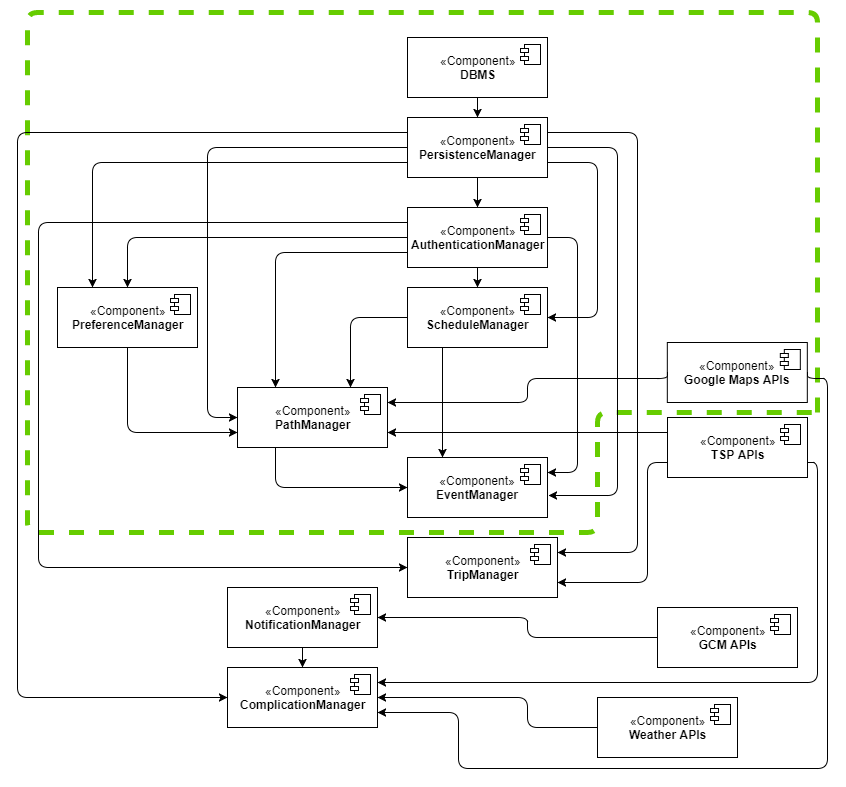
\includegraphics[scale=0.4]{app_server_I&T.png}
	\end{center}
\caption{ ApplicationServer - Actually tested subsystems subsystems}
\end{figure}
\newpage \noindent
For what concerns the Android App subsystem we have tested the DAOs that interact with the local DB. These tests can be found in test/java/it/polimi/travlendarplus, as can be seen in the previous chapter (see section 4.1).

\section{Procedure Adopted}
\subsection{Persistence Manager (JPA - DBMS interaction): Arquillian}
In order to perform our \textit{PersistenceManager}'s testing we have adopted the following procedure: we have exploited Arquillian features to obtain a testing configuration that allow us to use a testing container of GlassFish that can run and connect to an embedded GlassFish 3.1 instance.
Our \textit{PersistenceManager}'s tests simply  persist a set of sample entities to the database, connected with the GlassFish container, and then retrieve them using JPA Criteria API.
Each test method checks that the sample data retrieved from the database is correct. Before and after a test is performed, the database is cleaned up, in order to guarantee that each test is run in a clean environment.
This is the outcome of these tests:
\begin{figure}[H]
	\begin{center}
		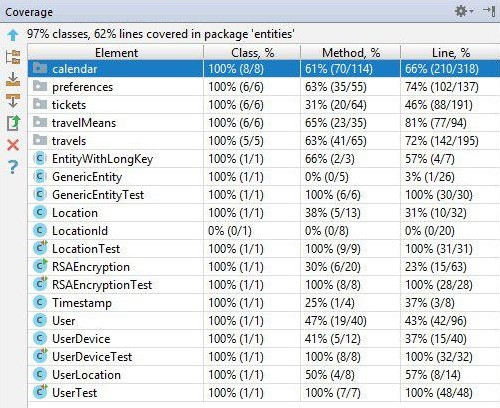
\includegraphics[scale=0.7]{JPA_test_outcome.jpg}
	\end{center}
\caption{ \textit{PersistenceManager} - code coverage}
\end{figure}

\subsection{Enterprise Java Beans: Mockito}
We used Mockito to test the \textit{PathManager}, a Stateless EJB that requires other Stateless EJBs (\textit{ScheduleManager} and \textit{PreferenceManager}) in order to perform its tasks. Using Mockito, all the functions performed by one of the injected beans were mocked: the idea is to consider these functions as working and to test the instructions properly defined in the \textit{PathManager}. 
\newpage
\noindent
In particular, we mocked \textit{ScheduleManager} functions in this way:
\begin{itemize}
	\item for each function that returns an event a predefined event is returned, depending on the parameter passed to the function;
	\item for \textit{PathCalculation} function a random response is returned, based on the travels passed to the function;
	\item for save functions a \textit{doNothing} method is used.
\end{itemize}  
\textit{PreferenceManager} functions are mocked in this way:
\begin{itemize}
	\item \textit{checkConstraints} function return always \textit{true};
	\item \textit{findBestPath} function always return the first element in the array of possibilities.
\end{itemize}
The most challenging functionalities that our system offers are the calculation of feasible paths, related to the events, that respect the user's constraints and  the possibility to force not scheduled events into the user's schedule. \\ \\
\textit{CalculatePath} function, for a given event, returns the path that allows the user to reach his event and the path that allows him to reach also the following one, according to the commitments in the schedule. \\
We considered a general case in which both previous and following events exist and we verified that:

\begin{itemize}
	\item when an event is inserted and the allotted time between the previous event and the inserted one is enough, we expect to obtain a feasible path;
	\item when an event is inserted and the allotted time between the inserted event and the following one is enough, we expect to obtain a feasible path;
	\item when an event's preference asks that the feasible path starts from the precedent user's location (location of the previous event), we expect to obtain a path that starts form there;
	\item when an event's preference asks that the feasible path starts from a given location (specified by the user) we expect to obtain a path that starts form there;
	\item for every obtained path, related to a given event, we always expect that the path's ending location is the same as the event's location.
\end{itemize}
\noindent
All the previous test cases are checked for the inserted event and its following one (since, when an event is inserted, the following path can change). When a following event does not exist the following path does not exist and so it has not to be checked. \\ \\
\noindent
We tested also \textit{swapEvents} function, a function that forces an overlapping event into the schedule and removes from the schedule all the events in conflict with the added one. \\
We verified the right behavior of the function in the following cases:
\begin{itemize}
	\item when the forced event overlaps with another one, the latter has to be removed from the schedule;
	\item when the forced event's path overlaps with another event, the conflicting event has to be removed from the schedule;
	\item when the forced event is inserted into the schedule and the following one is too close in time (and so a feasible path does not exist anymore), the following one has to be removed from the schedule;
	\item when the forced event is inserted into the schedule and it overlaps with a break event, but its minimum time is still guaranteed, the break event must remain into the schedule;
	\item when the forced event is inserted into the schedule and it overlaps with a break event, whose minimum time is no more guaranteed, the break event must be removed from the schedule. \\
\end{itemize}
We used Junit in order to test the beans that do not contain components difficult to be tested.
\begin{figure}[H]
	\begin{center}
		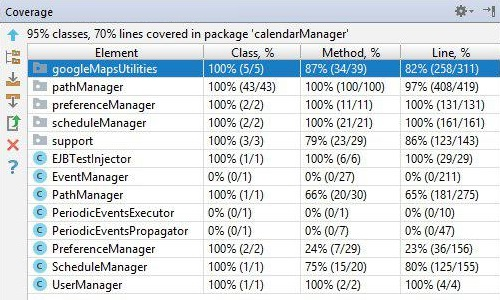
\includegraphics[scale=0.7]{CalendarManager_test_outcome.jpg}
	\end{center}
\caption{ textit{CalendarManager} - code coverage}
\end{figure}

\subsection{RESTful API Postman}
In order to test our RESTful APIs we have performed our requests using a useful software tool: Postman. This software tool allowed us to build API requests and see their outcome, checking that:
\begin{itemize}
	\item all invalid (due to wrong message format) requests are refused;
	\item all requests that try to access secured resources without being authenticated (with a token) receive an unauthorized response message;
	\item all requests with a right message format, but with invalid syntax, receive a bad request response message;
	\item all the correct requests gets replied with the correct response message. 
\end{itemize}
(For additional info about our RESTful API please refer to our relative documentation \href{httpsdocumenter.getpostman.comview2934379travlendar-restful-api7Log3CL}{\color{blue}link}).



	
	\chapter{INSTALLATION INSTRUCTIONS}
	\label{ch:INSTALLATION INSTRUCTIONS}	
		\section{Application Server and DBMS}
\label{sect:Application Server and DBMS}
\todo{TODO}

\section{Android App}
\label{sect:Android App}
This section contains a short guide to proper install and test the software required to run Travlendar+'s Android App.\\

 
\subsection{Instructions to run the App on your computer (recommended)}
\label{subsect:Android App}
\begin{itemize}
	\item Open your browser and head to \href{https://developer.android.com/studio/index.html}{\color{blue}https://developer.android.com/studio/index.html};
	\item Click on the 'Download Android Studio' green button;
	\item Accept the license agreement ( check the box that states 'I have read and agree with the above terms and conditions';
	\item Click on the 'Download Android Studio for <your OS name>' blue button (NB <your OS name> represent the name of your Operating System);
	\item The download process should automatically start and your browser should redirect you on the 'Install Android Studio' web page, if not head to: \href{https://developer.android.com/studio/install.html}{\color{blue}https://developer.android.com/studio/install.html};
	\item Follow the instructions relative to your OS;
	\item At the end of the installation process a Android Studio shows a window named 'Welcome to Android Studio', click on 'Profile or debug APK';
	\item Select Travlendar+'s APK location \todo{TODO};
	\item (close tip of the day) \todo{TODO};
	\item On the menu bar click on tools -\textgreater Android -\textgreater ADV manager;
	\item Click on 'Create Virtual device...' button;
	\item Select 'Phone as category' and then 'Pixel 2 XL';
	\item Click Next;
	\item Select Oreo system image (Android 8.0);
	\item Click on the download link on the right of 'Oreo' in order to download the selected android OS, and wait until the download ends; \todo{TODO}
	\item Click Next;
	\item Click Finish;
	\item Close the 'Android Virtual device Manager' window;
	\item On the menu bar click on Run -\textgreater Run ..... \todo{TODO};
	\item Select 'Pixel 2 XL API 26' virtual device;
	\item Wait until your Android virtual device starts;
	\item Enjoy Travlendar+'s Android App.	
\end{itemize}
	
	\chapter{EFFORT SPENT}
	\label{ch:EFFORT SPENT}
		\section{Pietro Melzi}
\begin{table}[H]
	\begin{tabular}{ p{2cm} p{10cm} p{3cm}}
	Date & Task & Hours of work\\
	\hline
	06/11/17 & Group session - Overall architecture proposed by Salvadore & 1 \\
	09/11/17 & Group session - Discussion on architecture components & 1 \\
	11/11/17 & Group session - Requirements traceability, considerations on sequence diagrams and other parts of document's section two & 8 \\
	12/11/17 & Sequence diagrams written on paper & 2 \\
	13/11/17 & Group session - Sequence diagrams written with software, discussion on algorithms & 7 \\
	14/11/17 & Considerations on sequence diagrams and requirements traceability, security algorithm on paper & 3 \\
	15/11/17 & Considerations on other algorithms with Salvadore & 1 \\
	18/11/17 & Group session - Encryption, univocal code and local DB updating algorithms, general considerations & 8 \\
	19/11/17 & Corrections in the document, description of calendar interface components & 5 \\
	20/11/17 & Group session - Fixes on component interfaces and sequence diagrams & 2 \\
	25/11/17 & Group session - ... & 0 \\
	\end{tabular}
\end{table}

\section{Alessandro Pina}
\begin{table}[H]
	\begin{tabular}{ p{2cm} p{10cm} p{3cm}}
	Date & Task & Hours of work\\
	\hline
	06/11/17 & Group session - Overall architecture proposed by Salvadore & 1 \\
	09/11/17 & Group session - Discussion on architecture components & 1 \\
	11/11/17 & Group session - ... & 8 \\
	13/11/17 & Group session - ... & 7 \\
	18/11/17 & Group session - ... & 8 \\
	20/11/17 & Group session - ... & 2 \\
	25/11/17 & Group session - ... & 0 \\
	\end{tabular}
\end{table}

\section{Matteo Salvadore}
\begin{table}[H]
	\begin{tabular}{ p{2cm} p{10cm} p{3cm}}
	Date & Task & Hours of work\\
	\hline
	06/11/17 & Group session - Overall architecture proposed by me & 1 \\
	09/11/17 & Group session - Discussion on architecture components & 1 \\
	11/11/17 & Group session - ... & 8 \\
	13/11/17 & Group session - ... & 7 \\
	18/11/17 & Group session - ... & 8 \\
	20/11/17 & Group session - ... & 2 \\
	25/11/17 & Group session - ... & 0 \\
	\end{tabular}
\end{table}
		
	\chapter{REFERENCES}
	\label{ch:REFERENCES}
	
		\section{Bibliography}
		\label{sect: Bibliography}
		\begin{enumerate}[(I)]
	\item \href{https://javaee.github.io/glassfish/doc/5.0/release-notes.pdf}{\color{blue}GlassFish Server Open Source Edition - Release Notes - Release 5.0}
	\item \href{https://javaee.github.io/glassfish/doc/5.0/installation-guide.pdf}{\color{blue}GlassFish Server Open Source Edition - Installation Guide - Release 5.0 }
	\item \href{https://javaee.github.io/glassfish/doc/5.0/installation-guide.pdf}{\color{blue}GlassFish Server Open Source Edition - Installation Guide - Release 5.0 }
	\item Document provided in beep course web page in slides folder: "JEE Tools Instructions for Lab";
\end{enumerate}
		
		\section{Software used}
		\label{sect: Software used}
		This document is written in LaTex, a markup language used for text editing, and includes sections realized with different software tools. Here we show the list of used software:
\begin{itemize}
	\item Texmaker 5.0.2 (compiled with Qt 5.8.0) for writing the document;
	\item StarUML 2.8.0 for class diagram, use cases diagrams and sequence diagrams;
	\item draw.io for model of shared phenomena and statechart diagram;
	\item Mockplus 3.2.6 for mockups;
	\item Alloy Analyzer 4.2 for the creation of the model.	
\end{itemize}
		

\end{document}
